\documentclass{beamer}

\mode<presentation>
{
  \usetheme{Madrid}
  \usecolortheme{rose}
  \usefonttheme{structurebold}
  \setbeamertemplate{navigation symbols}{}
  \setbeamertemplate{caption}[numbered]
}

\usepackage[english]{babel}
\usepackage[utf8x]{inputenc}
\usepackage{listings}
\usepackage{inconsolata}
\usepackage{qrcode}

\usepackage{tikz}
\usetikzlibrary{arrows.meta, positioning}

\usepackage{upquote}

\lstset{
  basicstyle=\ttfamily\small,
  breaklines=true,
  columns=fullflexible,
  frame=single,
  showstringspaces=false
}

\title[Take Control of Your Build with Mill]{Take Control of Your Build:\\Spring Boot and Beyond with Mill}
\author{Vasilis Nicolaou}
\institute{Vaslabs LTD}
\date{CERN @ 02 December 2025}

\begin{document}

% =========================
% Title & Agenda
% =========================

\begin{frame}
  \titlepage
\end{frame}

\begin{frame}{Outline}
  \tableofcontents
\end{frame}

% =========================
% Intro / Context
% =========================

\section{Introduction}

\begin{frame}{Who am I?}
  \begin{itemize}
    \item JVM developer (Java, Scala) with experience in distributed systems.
    \item Contributor to Mill, initially adding Android support and lately around Spring Boot.
    \item I went through various build tools; Maven, Gradle, Sbt and now... Mill!
    \item Today: Software Engineering Consultant with own firm and a small but strong team of software engineers!
  \end{itemize}
\end{frame}

% =========================
% Live Demos First
% =========================

\section{Mill in Action}

\subsection{Demo 1: Spring Boot with Mill}

\begin{frame}[fragile]{Demo 1: A simple Spring Boot project}
  \vspace{0.5em}
  \textbf{Quick Mill setup commands:}
  \begin{lstlisting}[language=bash, basicstyle=\ttfamily\tiny]
url=https://repo1.maven.org/maven2/com/lihaoyi/mill-dist/1.1.0-RC2-40-0576e4/mill-dist-1.1.0-RC2-40-0576e4-mill.sh
curl -L "${url}" -o mill
chmod +x mill
./mill version
\end{lstlisting}
\end{frame}

\begin{frame}[fragile]{Sample Mill build for Spring Boot}
  \begin{lstlisting}[language=Scala]
package build
import mill.*, mill.javalib.*

object `package` extends MavenModule { outer =>
  override def bomMvnDeps = Seq(
    mvn"org.springframework.boot:spring-boot-dependencies:3.5.7"
  )
  override def mvnDeps = Seq(
    mvn"org.springframework.boot:spring-boot-starter-web"
  )

  object test extends MavenTests, TestModule.Junit5 {
    override def bomMvnDeps = outer.bomMvnDeps()
    override def mvnDeps =
      Seq(mvn"org.springframework.boot:spring-boot-starter-test")
  }
}
  \end{lstlisting}
\end{frame}

\begin{frame}[fragile]{Spring Boot + Fmt}
  \begin{lstlisting}[language=Scala]
package build
import mill.*, mill.javalib.*, palantirformat.PalantirFormatModule
object `package` extends MavenModule,PalantirFormatModule
  \end{lstlisting}
  \vspace{0.5em}
  \textbf{Or without build code changes}
  \begin{lstlisting}[language=Bash]
   ./mill mill.javalib.palantirformat.PalantirFormatModule/
  \end{lstlisting}

\end{frame}

\begin{frame}[fragile]{What's happening under the hood?}
\begin{lstlisting}[language=Bash]
./mill visualizePlan compile
\end{lstlisting}
\end{frame}

\subsection{Demo 2: AOT and GraalVM}

\begin{frame}{Demo 2: Spring Boot AOT + GraalVM}
  \begin{itemize}
    \item Recently merged support in Mill for:
      \begin{itemize}
        \item Spring Boot AOT processing.
        \item Building native images with GraalVM.
      \end{itemize}
  \end{itemize}
\end{frame}

\begin{frame}[fragile]{Demo 2: Spring Boot AOT + GraalVM}
  \begin{lstlisting}[language=Scala]
package build
import mill.*, mill.javalib.*, spring.boot.SpringBootModule

object `package` extends SpringBootModule, MavenModule {
  override def springBootPlatformVersion = "3.5.7"
  override def artifactName: T[String] = "spring-boot-native-demo"
  object prod extends SpringBootOptimisedBuildModule, MavenModule
  object native extends MavenModule, NativeSpringBootBuildModule {
    def jvmId = "graalvm-community:23.0.1"
  }
  def mvnDeps = 
    Seq(mvn"org.springframework.boot:spring-boot-starter-web")
  object test extends SpringBootTestsModule, MavenTests, 
        TestModule.Junit5 {
    def mvnDeps =
      Seq(mvn"org.springframework.boot:spring-boot-starter-test")
  }
}
  \end{lstlisting}
\end{frame}

% =========================
% Mill Design / Concepts
% =========================

\section{How Mill Works Under the Hood}

\begin{frame}{Mill design principles}
  \begin{itemize}
    \item Build definitions are Scala code:
      \begin{itemize}
        \item Uses best world of OOP and FP.
        \item Easily refactorable and testable; each Task yields a value that can be inspected, cached, reused.
      \end{itemize}
    \item Task graph is generated automatically and is inspectable.
      \begin{itemize}
        \item No need to worry about caching or cleaning up task directories or task files
        \item No need to declare dependencies between tasks.
      \end{itemize}
    \item Modules are composable units:
      \begin{itemize}
        \item Inheritance and composition instead of copy-paste.
      \end{itemize}
  \end{itemize}
\end{frame}

\begin{frame}[fragile]{Demo: Add Task, inspect its directory and value}
  \begin{lstlisting}[language=Scala]
trait FileCounterMavenModule extends MavenModule {

  def countAllSourceFiles: T[Int] = Task {
    allSourceFiles().filter(p => os.isFile(p.path)).size
  }

  def allGeneratedSourceFiles: T[Seq[PathRef]] = Task {
    generatedSources().flatMap(p => 
        os.walk(p.path).filter(os.isFile(_))
    ).map(PathRef(_))
  }

  def countGeneratedSourceFiles: T[Int] = Task {
    allGeneratedSourceFiles().size
  }
}
  \end{lstlisting}
\end{frame}

% =========================
% Spring Boot specifics
% =========================

\section{Annotation Processors}

\begin{frame}{Java annotation Processors}
  \begin{itemize}
    \item Recently added support for easily adding annotation processors in Mill.
    \item Annotation processor dependency resolution also takes into account Maven BOMs.
    \item Useful for Spring Boot configuration metadata generation, Lombok, AutoValue, Dagger, Immutables, etc.
    \item Example: \url{https://mill-build.org/mill/javalib/web-examples.html\#_micronaut_hello_world_app}
  \end{itemize}
\end{frame}

\begin{frame}{Kotlin: KSP support}
  \begin{itemize}
    \item Kotlin Symbol Processing(KSP) support was added as part of the ongoing efforts to add Android support in Mill.
    \item Can be used for both Kotlin and Android projects.
    \item Micronaut example: \url{https://mill-build.org/mill/kotlinlib/web-examples.html\#_micronaut_app}
    \item Dagger example: \url{https://mill-build.org/mill/kotlinlib/module-config.html\#_dependency_injection_with_dagger_and_ksp}
  \end{itemize}
\end{frame}

% =========================
% Android as Stress Test
% =========================

\section{Android}

\subsection{Mill Under Extreme Conditions}

\begin{frame}{Android support shows how well designed Mill is}
  \begin{itemize}
    \item My first experience with Mill was to add support for Android builds: \url{https://github.com/com-lihaoyi/mill/pull/4169}
    \item We've developed the basic feature set for the dev lifecycle and got it merged within 2 weeks.
    \item About a year since, Mill supports all kinds of complex Android configurations out of the box.
    \item Android builds are:
      \begin{itemize}
        \item Multi-stage (resources (compiling, linking), manifests, dexing, packaging).
        \item Tooling-heavy and configuration-heavy.
      \end{itemize}
    \item If a build tool can handle Android cleanly:
      \begin{itemize}
        \item It has the right design foundations 
        \item It’s a good sign it can handle complex pipelines
      \end{itemize}
  \end{itemize}
\end{frame}

%To be continued...

\begin{frame}[fragile]{High-level Android pipeline in Mill (conceptual)}
  \centering
  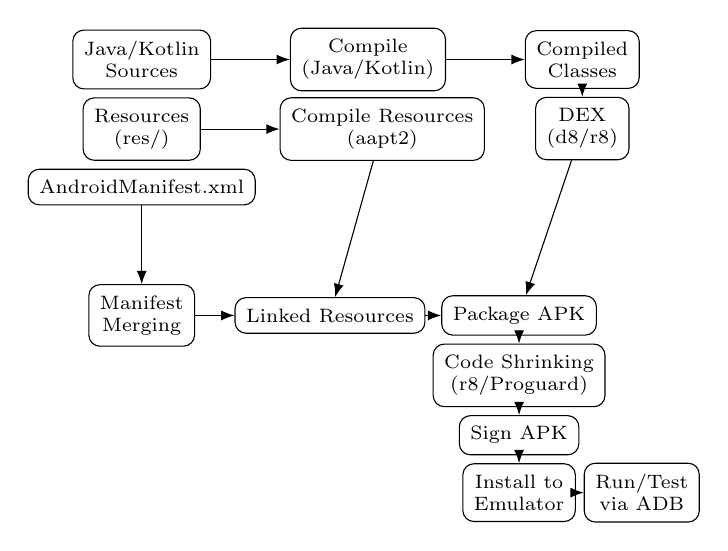
\begin{tikzpicture}[
    node distance=0.1cm,
    every node/.style={
      rectangle,
      draw,
      rounded corners,
      align=center,
      inner sep=4pt,
      font=\scriptsize
    },
    >=LaTeX
  ]

    % Left column: inputs
    \node (src) {Java/Kotlin\\Sources};
    \node (res) [below=of src] {Resources\\(res/)};
    \node (man) [below=of res] {AndroidManifest.xml};

    % Middle column: processing
    \node (cjava) [right=1cm of src] {Compile\\(Java/Kotlin)};
    \node (cres)  [right=1cm of res] {Compile Resources\\(aapt2)};
    \node (mmerge)[below=1cm of man] {Manifest\\Merging};

    \node (linked) [right=0.5cm of mmerge] {Linked Resources};

    % Right column: classes / dex / packaging
    \node (classes) [right=1cm of cjava] {Compiled\\Classes};
    \node (dex)     [below=of classes] {DEX\\(d8/r8)};
    \node (pack)    [right=0.2cm of linked] {Package APK};
    \node (shrink)  [below=of pack] {Code Shrinking\\(r8/Proguard)};
    \node (sign)    [below=of shrink] {Sign APK};
    \node (install) [below=of sign] {Install to\\Emulator};
    \node (run)     [right=of install] {Run/Test\\via ADB};

    % Edges
    \draw[->] (src) -- (cjava);
    \draw[->] (res) -- (cres);
    \draw[->] (man) -- (mmerge);

    \draw[->] (mmerge) -- (linked);
    \draw[->] (cres)   -- (linked);

    \draw[->] (cjava)  -- (classes);
    \draw[->] (classes) -- (dex);

    \draw[->] (linked) -- (pack);
    \draw[->] (dex)    -- (pack);

    \draw[->] (pack)   -- (shrink);
    \draw[->] (shrink) -- (sign);
    \draw[->] (sign)   -- (install);
    \draw[->] (install)-- (run);

  \end{tikzpicture}
\end{frame}

\begin{frame}{Visualizing the task graph for androidApk}
  \includegraphics[scale=0.045]{jetnews_visualise_plan}
\end{frame}

\begin{frame}{Spring Boot native.nativeImage comparison}
    \includegraphics[scale=0.045]{springboot_native_visualise}
\end{frame}
% =========================
% Comparison & Wrap-up
% =========================

\section{Closing Remarks}

\subsection{Key Takeaways}

\begin{frame}{Key Takeaways}
  \begin{itemize}
    \item Mill treats builds as real code, not opaque configuration (but if you wish, you can also use the latter with YAML (new)).
    \item The task graph is explicit, inspectable, and composable.
    \item Spring Boot and AOT/GraalVM support show Mill’s power for modern JVM apps.
    \item Android support demonstrates that Mill scales to highly complex build pipelines.
    \item You can take control of your build by easily understanding and extending it.
  \end{itemize}
\end{frame}

\subsection{Q\&A}

\begin{frame}{Questions}
  \begin{itemize}
    \item Which version of Spring boot are you using?
    \item What is your library stack? (Mono/Flux, rxJava, Lombok, Immutables)
    \item Do you deploy native images? Are you using AOT?
    \item Any other testing libraries/pre-processors?
    \item What is the biggest pain on the build tool you are using?
    \item Plain Java? Kotlin? Mixed?
  \end{itemize}
\end{frame}

\begin{frame}{Thank you!}
  \centering
  \Large{Thank you!}\\[1em]
  \normalsize
  \begin{itemize}
      \item Documentation: \url{https://mill-build.org/}
      \item Github Repo: \url{https://github.com/com-lihaoyi/mill}
      \item Try Mill and join Mill's Discord Channel:
  \end{itemize}

  \quad
  \qrcode[height=5cm]{https://discord.gg/bt3DPbfUmV}

\end{frame}

\end{document}
